\section{Das HTTP-Protokoll}

Bei webbasierten Anwendungen wird die Client-Seite durch einen Web-Browser realisiert, auf der Server-Seite wird ein Web-Server wie bspw. \textit{Apache Tomcat}\footnote{
    \url{https://tomcat.apache.org} - abgerufen 3.2.2024
} benutzt.\\

\noindent
Der Web-Server liefert statische Dateien aus oder Seiten, die Programmcode enthalten, der auf dem Client ausgeführt wird (bspw. \textit{JavaScript}).\\

\noindent
Der Client kann auch über den Server ausgeführte Programme anfordern, die entsprechende Daten für den Client generieren, wie bspw. \textbf{Servlets}.\\

\noindent
Um mit einem Server zu kommunizieren, baut der Client über \textbf{TCP} eine Verbindung mit dem Server auf:\\
Über das \textbf{HTTP-Protokoll}\footnote{
Bestandteilt der Anwendungsschicht - s. \url{https://en.wikipedia.org/wiki/HTTP} - abgerufen 3.2.2024
} werden dann Anfragen und Antworten zwischen Client und Server verhandelt; Antworten können über auf dem Server laufende Programme dynamisch generierte Seiteninhalte sein.\\

\noindent
\textbf{HTTP} (\textit{HyperTextTransferProtocol})\footnote{
    s. a. ``RFC 9110 HTTP Semantics``: \url{https://www.rfc-editor.org/rfc/rfc9110.html} - abgerufen 4.2.2024
} ist ein ASCII-Protokoll auf Schicht 5 und für die Vermittlung webbasierter Dienste gedacht.

\begin{figure}
    \centering
    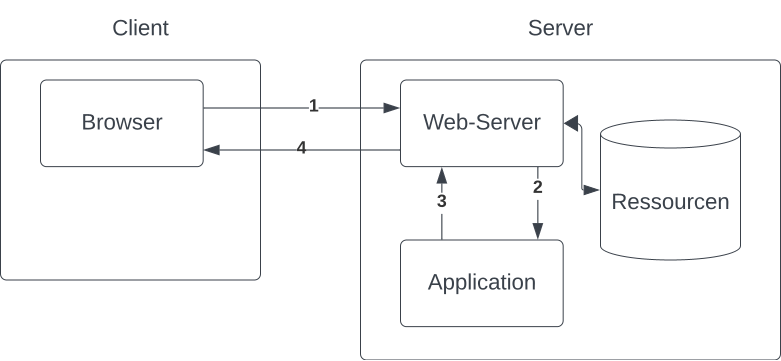
\includegraphics[scale=0.5]{chapters/fopt6/img/clientserver}
    \caption{Der Client erstellt über den Webbrowser eine TCP-Verbindung zu dem Webserver, wobei die Adressinformationen in der URL festgelegt sind.
    Der Webserver kann nun in seiner Antwort sowohl statische Ressourcen als auch dynamisch generierte Daten bereitstellen.
    Syntax und Semantik der Anfrage und Antwort ist über das HTTP-Protokoll definiert (Quelle: in Anlehnung an \cite[402, Bild 8.1]{Oec22})}
    \label{fig:clientserver}
\end{figure}

\subsection{GET}

Über eine \textbf{URL} (\textit{Universal Resource Locator}\footnote{
s. \url{https://en.wikipedia.org/wiki/URL} - abgerufen 3.2.2024
}) wird über den Browser eine Ressource angefordert.

\begin{tcolorbox}[enlarge top by=0.5cm,enlarge bottom by=0.5cm]
    Eine \textbf{URL} ist eine \textbf{URI} (\textit{Uniform Resource Identifier}\footnote{
        s. \url{https://en.wikipedia.org/wiki/Uniform_Resource_Identifier} - abgerufen 3.2.2024
    }) und enthält u.a. weitere Informationen zur Lokalisierung der Ressource - bspw. durch die Angabe des Protokolls, über das die Ressource beschafft werden soll\footnote{s. ``RFC 3986 - 1.1.3.  URI, URL, and URN``: \url{https://datatracker.ietf.org/doc/html/rfc3986#section-1.1.3} - abgerufen 3.2.2024}.
\end{tcolorbox}

\noindent
Der an den Server übermittelte \textbf{GET}-Request besteht aus der Angabe der angeforderten Ressource und dem Protokoll, das verwendet wird:

\begin{minted}[]{http}
GET /resource.html HTTP/1.1
\end{minted}
\\

$\rightarrow$ Ein \textbf{GET}-Request besteht aus beliebig vielen Zeilen.
Mit einer Leerzeile wird das Ende des Request angezeigt.\\

\noindent
Eine \textbf{HTTP-Response} enthält wieder Kopfdaten (\textbf{Header}) und den \textbf{Body}, der leer sein kann.\\
Header und Body sind durch eine Leerzeile voneinander getrennt\footnote{
    s. \url{https://www.rfc-editor.org/rfc/rfc7230#section-3} - abgerufen 3.2.2024
}.\\
Weitere Leerzeilen im Body haben keine weitere Bedeutung für das Protokoll und gehören zum Inhalt der angeforderten Ressource.\\

\noindent
Der Client kann weitere Daten anfordern, bspw. wenn in der ausgelieferten HTML-Seite Bilder oder andere statische Ressourcen vorkommen.\\
Bei \textbf{HTTP/1.0} muss der Client für jede Ressource eine neue \textbf{TCP}-Verbindung aufbauen.\\
Nutzt der Client hingegen \textbf{HTTP/1.1}, hält der Server genau diese Verbindung offen.
Über diese Verbindung kann der Client weitere Daten anfordern.

\begin{itemize}
    \item Bei der Verwendung von \textbf{HTTP/1.1} muss außerdem in der zweiten Zeile der Anfrage der Zielhost stehen, damit ein Server, der {ggf.} mehrere Domains hostet, die Anfrage an die richtige Domain weiterleitet\footnote{s. ``RFC 7320 - 5.4.  Host``: \url{https://www.rfc-editor.org/rfc/rfc7230#section-5.4} - abgerufen 3.2.2024}.
    \begin{minted}[]{http}
GET /index.php HTTP/1.1
Host: www.conjoon.org
    \end{minted}
    \item Wird der Header \textit{Connection: keep-alive}\footnote{
    s. ``RFC 2068 - 19.7.1 Compatibility with HTTP/1.0 Persistent Connections``: \url{https://www.rfc-editor.org/rfc/rfc2068#section-19.7.1} - abgerufen 3.2.2024
    } mitgesendet, teilt der Client dem Server mit, dass die Verbindung zum Herunterladen weiterer Daten geöffnet bleiben soll.
    \item Bei einer HTTP-Response weist die Antwort-Zeile \textit{Connection: close} daraufhin, dass die Verbindung nicht persistent ist und mit der Bearbeitung der Antwort geschlossen wird\footnote{
    s. ``RFC 2068 - 14.10 Connection``: \url{https://www.rfc-editor.org/rfc/rfc2068#section-14.10} - abgerufen 3.2.2024
    }.
\end{itemize}

\subsection{Formulare in HTML}

\textit{<form>...</form>} wird für Formulare in HTML genutzt, in \textit{action} steht die URL, an der die Formulardaten gesendet werden sollen, mit \textit{method} kann man die HTTP-Methode angeben, die zum Senden des Formulars genutzt werden soll\footnote{
s. ``<form>: The Form element``:\url{https://developer.mozilla.org/en-US/docs/Web/HTML/Element/form} - abgerufen 3.2.2024
}.\\

\noindent
\textbf{radio}-inputs erhalten alle dasselbe \textit{name}-Attribut, um sie zu einer Gruppe zusammenzuführen.\\

\noindent
Fehlt für eine \textbf{checkbox} die Selektion, wird sie bei der Übertragung der Formulardaten nicht berücksichtigt.
Ist das \textit{value}-Attribut für die Checkbox gesetzt und wurde die Checkbox selektiert, enthalten die Request-Daten den Inhalt von \textit{value}, ansonsten standardmäßig den Wert \textit{on}:

\blockquote[{\url{https://developer.mozilla.org/en-US/docs/Web/HTML/Element/input/checkbox} - abgerufen 3.2.2024, Hervorherbungen ausgelassen}]{
    If the value attribute was omitted, the default value for the checkbox is on, so the submitted data in that case would be subscribe=on.
}

\subsection{POST}

Nutzt man \textbf{GET} zur Übermittlung von Formulardaten, werden die Daten als Query-String an die URL gehangen.\\

\noindent
\textbf{POST} schickt die Formulardaten im Body an die in \textit{action} angegebene URL.

\begin{itemize}
    \item Vorteile \textbf{GET}: Formulardaten können mit der URL gespeichert werden, bei \textbf{POST} geht das nicht, da diese im Body verborgen sind
    \item Nachteile \textbf{GET}: bei \textbf{GET} ist die Länge der eingegebenen Formulardaten begrenzt, bei \textbf{POST} nicht.
    \begin{tcolorbox}[colback=red!20,color=white,title=Anmerkung]
    Die Aussage bzgl. der Begrenzung von \textbf{GET/POST} findet sich in \cite[409]{Oec22}.\\
    Tatsächlich ist die Länge nicht begrenzt per Spezifikation\footnote{``RFC 7230 - 3.1.1.  Request Line``: \url{https://datatracker.ietf.org/doc/html/rfc7230#section-3.1.1} - abgerufen 3.2.2024}. \\
    Es wird aber empfohlen, Request URIs abzuweisen, die zu lang sind\footnote{siehe bspw. ``RFC 2616 - 10.4.15 414 Request-URI Too Long``: \url{https://datatracker.ietf.org/doc/html/rfc2616#section-10.4.15} - abgerufen 3.2.2024
    }.\\
    Auch für \textbf{POST} wird in den Spezifikationen keine max. Länge vorgegeben.
    Allerdings kann die max. akzeptierte Länge des Bodys eines POST-Requests durch den Web-Server begrenzt werden\footnote{
        ``RFC7231 - 6.5.11.  413 Payload Too Large``: \url{https://www.rfc-editor.org/rfc/rfc7231#section-6.5.11} - abgerufen 3.2.2024
    }.\\
    Beides ist sinnvoll, um einer Überlastung des Webservers durch zu große Anfrage-Längen vorzubeugen.
    \end{tcolorbox}
\end{itemize}

\subsection{Format von HTTP-Anfragen und -Antworten}

Eine HTTP-Anfrage hat grundsätzlich folgende Struktur\footnote{
Es ist grundsätzlich möglich, bei GET-Requests den Body mitzuschicken.
    Allerdings rät RFC 9110 davon ab: ``A client \textbf{SHOULD NOT} generate content in a GET request unless it is made directly to an origin server that has previously indicated, in or out of band, that such a request has a purpose and will be adequately supported. An origin server \textbf{SHOULD NOT} rely on private agreements to receive content, since participants in HTTP communication are often unaware of intermediaries along the request chain.`` (Hervorhebungen i.O., \url{https://www.rfc-editor.org/rfc/rfc9110#section-9.3.1-6} - abgerufen 3.2.2024)
}:

\begin{minted}[]{text}
<methode> <uri> HTTP/<version>
<headername>: <headerwert>
...
<headername>: <headerwert>
<newline>
<body>
\end{minted}

Die Antwort sieht i.A. folgendermaßen aus:

\begin{minted}[]{text}
HTTP/<version> <StatusCode> <StatusText>
<headername>: <headerwert>
...
<headername>: <headerwert>
<newline>
<body>
\end{minted}

\subsection*{``Content-Length`` Header}
Bei \textbf{POST} nutzt der Server die Verbindung, die der Client zur Anfrage aufgebaut hat, um die Antwort zu senden.\\
Der Server muss wissen, wann er den kompletten Datenteil gelesen hat, bevor er mit der Antwort beginnt.\\
Bis zum Verbindungsende kann nicht gelesen werden, sonst kann keine Antwort gesendet werden.\\
Trennzeichen sind für den Body nicht ausgemacht.\\
Nach $n$-Zeichen, die der Client im Header über \textbf{Content-Length} spezifiziert, geht der Server davon aus, dass die Anfrage nach der Leerzeile (Trennzeichen Header / Body) genauso viele Daten enthält.\\
Sind diese $n$ Daten gelesen, beginnt der Server mit der Aufbereitung der Antwort an den Client\footnote{
s.a. Skript FOPT6 Übung 14.2
}.

